\documentclass[12pt,a4paper]{article}
\usepackage{arial}
\usepackage{graphicx}
\usepackage{subfigure}
\usepackage{amssymb,amsmath,amsfonts}
\usepackage[utf8]{inputenc}
\usepackage[spanish]{babel}
\graphicspath{{imagenes/}}
\usepackage{geometry}
\newcommand{\tabitem}{~~\llap{\textbullet}~~}
\usepackage{caption}
%\oddsidemargin = -.3cm
%\textwidth = 17cm
%\textheight = 24cm
%\headsep = 0cm
\renewcommand{\baselinestretch}{1.5}
\geometry{a4paper,left=2cm,right=2cm,top=2cm,bottom=2cm}


 
\begin{document}
\renewcommand{\listtablename}{Indice de tablas}
\renewcommand{\tablename}{Tabla}
\begin{titlepage}

    \begin{figure}[h]
 	\centering
    	{
\includegraphics[height=2cm]{SEP_logo}}
    	\hspace{6cm}
    	{
\includegraphics[height=2cm]{TecNM}}
    \end{figure}
    
    \centering
    \vspace{1cm}
    {\Large\bfseries Instituto Tecnológico de Ciudad Guzmán\par \vspace{.5cm}}
    {\Large \scshape Departamento de Ingeniería Eléctrica y Electrónica \par \vspace{.5cm}}
    {\Large \scshape Ingeniería Electrónica \par \vspace{.5cm}}
    \begin{figure}[h]
    \centering
     %
\includegraphics[height=3cm]{Logo_Ing_Electronica} \hspace{1cm}
     \includegraphics[height=4cm]{logo}
     %
\includegraphics[height=3cm]{electronica}
    \end{figure}
    \par \vspace{.2cm}
   
	{\huge Microcontroladores\par\vspace{.5cm}}
	{\Large\bfseries Investigación\\ \par\vspace{3cm}}
	
	\flushright{
	{\large{\itshape Juan José Carranza García }\hspace{1cm}NC. 15290337\par}
	\vspace{1cm}
	\centering
	{\large Catedrático\par
	Dr.Francisco Ochoa Cardenas\par\vspace{1cm}}
	\flushright
	{\large Cd. Guzmán, Jalisco,. 11 de abril del 2018\par}}
\end{titlepage} 

   \newpage
   
   
   \begin{center}
    \textbf{\textit{Introducción}}
   \end{center}
   En el siguiente trabajo se buscara introducir al lector en el amplio mundo de los microcontroladores, se abordaran conceptos tecnicos del microcontrolador asi como la arquitectura con la que estos trabajan.\\
   Se estudiaran los registros internos y se mencionara cual es el nombre y el proposito de cada uno de estos, se dara una introduccion al lenguaje ensamblador y se explicaran los primeros comandos basicos para poder realizar un programa dentro del IDE MPLAB para microcontroladores PIC, y se mostraran algunos simuladores, debugger y emuladores que existen para esta familia de circuitos integrados.\\
   A lo largo de la lectura, se observara la funcionalidad de cada una de las terminales del mirocontrolador pic16f887 , y se veran los encapsulados disponibles para este microcontrolador.
   
   \newpage
   \tableofcontents
   \newpage
   \listoffigures
   \newpage
   \listoftables
   \newpage
   \renewcommand{\figurename}{Figura 1.}
    \renewcommand{\tablename}{Tabla 1.}
   \setcounter{table}{0}
   \section{Introducción a la estructura de los microcontroladores}
   Un microcontrolador es una microcomputadora en un chip hecha por medio de fabricación VLSI (Very Large Scale Integration), este contiene un CPU (Central Processing Unit) , una memoria de programa y una de datos, puertos de entradas y salidas, y algunos otros componentes integrados en un solo chip, Figura\ref{fig:ComponentesMicrocontrolador}  \cite{Ravi}.
   
   \begin{figure}[htpb]
   \centering
   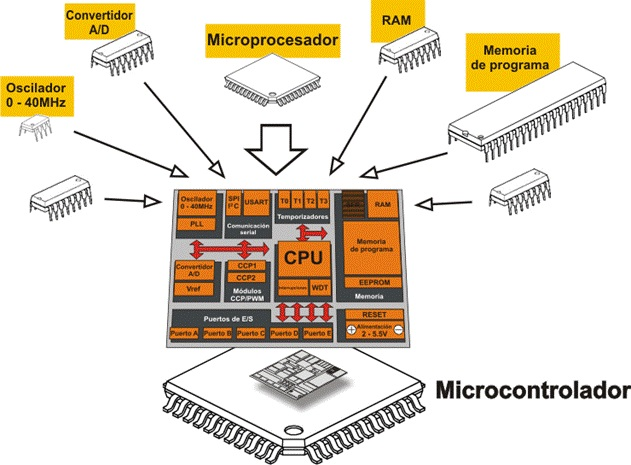
\includegraphics[height=7cm]{Figura1_1}
   \caption{Componentes Internos del Microcontrolador \cite{Ravi}}
   \label{fig:ComponentesMicrocontrolador}
   \end{figure}
   
   La mayoría de los microcontroladores modernos contiene más periféricos, como lo son SPI (Serial Peripheral Interface) , I2C (Inter Integrated Circuit), CAN (Controlled Area Network), USB (Universal Serial BUS), y muchos otros más. 
   
   \subsection{Conceptos básicos de los Microcontroladores}
   Los microcontroladores se pueden clasificar según 2 parámetros, de acuerdo con su función y de acuerdo a su longitud de palabra.\\
   De acuerdo a la función: se separan los microcontroladores de propósito general, los cuales contienen CPU, Memorias, E/S y algunas instrucciones no específicas, otros de los clasificados por función son los especializados, los cuales su arquitectura e instrucciones son orientadas hacia algún tipo de aplicación concreta, como lo puede ser comunicaciones, manejo de teclados, DSP, procesamiento de video, etc.De acuerdo con su longitud de palabra: existen microcontroladores de 4, 8, 16, 32 y 64 bits. La selección de la longitud de palabra depende de la aplicación que este tendrá, a continuación, se muestra una tabla (Tabla \ref{fig:TablaAplicaciones}) en la cual se muestran algunas aplicaciones y ejemplos de los microcontroladores utilizados para esa aplicación.
   
   \begin{table}[htpb]
   \centering
   \caption{Seleccion de microcontrolador y fabricante por Aplicacion \cite{Ravi}.}
    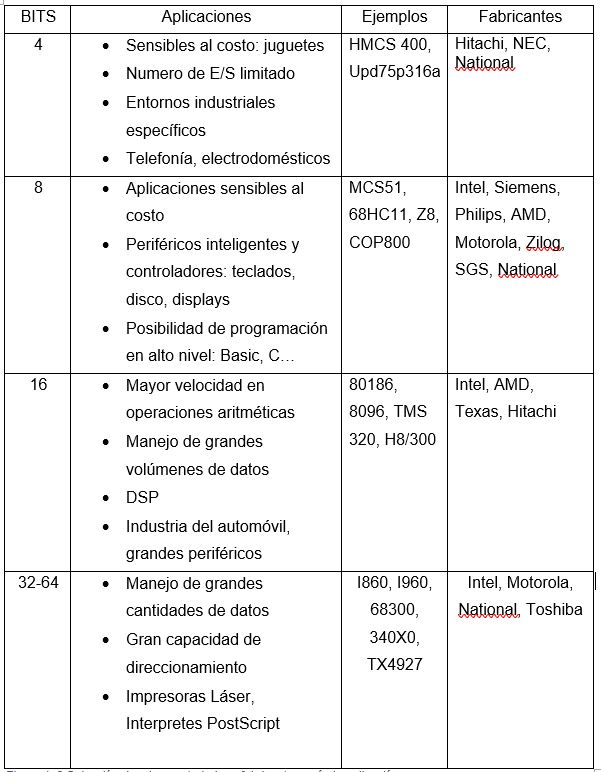
\includegraphics[height=20cm]{Tabla}
  
   \label{fig:TablaAplicaciones}
   \end{table}
   
 
  
   En la actualidad las familias de microcontroladores mas utilizados en la robótica competitiva son los microcontroladores PIC de microchip, los AVR de Atmel y los STM de STMicroelectronics.\\ 
   
   \textbf{Microcontroladores PIC} \\
   El nombre verdadero de este microcontrolador es PICmicro (Peripheral Interface Controller), conocido bajo el nombre PIC. Su primer antecesor fue creado en 1975 por la compañía General Instruments. Este chip denominado PIC1650 fue diseñado para propósitos completamente diferentes. Diez años más tarde, al añadir una memoria EEPROM, este circuito se convirtió en un verdadero microcontrolador PIC. Hace unos pocos años la compañía Microchip Technology fabricó la 5 billonésima muestra.\\
   
   Los PIC’s más utilizados son:
   \begin{itemize}
   \item PIC12C508/509: encapsulamiento reducido de 8 pines, oscilador interno, popular en pequeños diseños como el iPod remote
   \item PIC16F84: Considerado obsoleto, pero imposible de descartar y muy popular
   \item PIC16F84A : Buena actualización del anterior, algunas versiones funcionan a 20 MHz, compatible 1:1
   \item PIC12F629/675 PIC16F628 PIC16F88 : Nuevo sustituto del PIC16F84A con más memoria, oscilador interno, PWM, etc que podría convertirse en popular como su hermana menor). La familia PIC16F87X y PIC16F87XA (los hermanos mayores del PIC16F84 y PIC16F84A, con cantidad de mejoras incluidas en hardware. Bastante común en proyectos de aficionados)
   \item PIC18F2455 y similares con puerto USB 2.0 PIC18F2550 PIC18F452 PIC18F4550 dsPIC30F3011 (Ideales para control electrónico de motores eléctricos de inducción).
   \item PIC32 (Nueva gama de PIC de 32 bits).
   \end{itemize}
   
   \subsubsection{Diferencia entre Microcontrolador y Microprocesador}
   En la actualidad existen dos grandes tipos de chips en la industria, los microcontroladores y los microprocesadores, sin embargos por mas que estos sean semejantes físicamente, existen muchas diferencias entre ambos.\\
   Los microprocesadores tienen una arquitectura destinada al procesamiento de la información. Las características de estos son que contiene la CPU, la memoria RAM, ROM y los periféricos se encuentran separados de este a diferencia que en el microcontrolador \cite{Carva}.\\
   Los microcontroladores están destinados a funcionar casi independientemente, ya que contiene su CPU, la memoria RAM y ROM, puertos de E/S, timers, conversores A/D y D/A y algunos otros puertos de comunicaciones. \\
   La principal diferencia entonces se encuentra en que los microcontroladores ya contienen en si los periféricos para interactuar con el CPU y el microcontrolador necesita conectar estos de una manera externa, en la Figura  \ref{fig:ComponentesMicros} se muestra gráficamente esta diferencia.\\
   
   \begin{figure}[htpb]
   \centering
   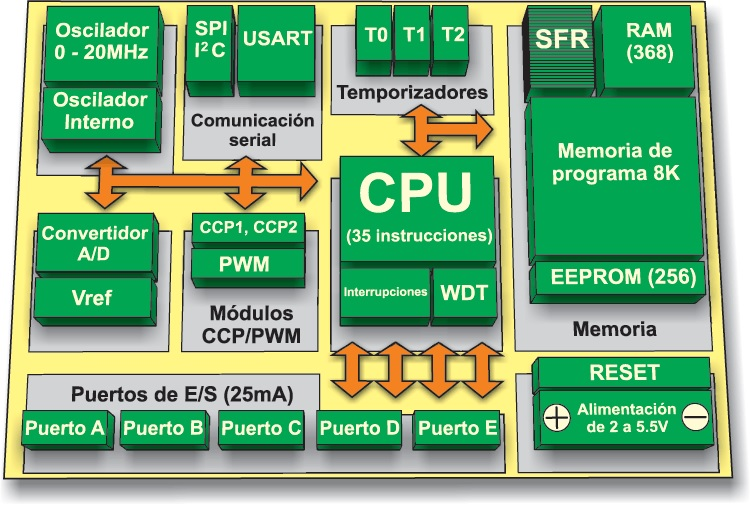
\includegraphics[height=4cm]{MicrocontroladorPartes}
   \hspace{1cm}
   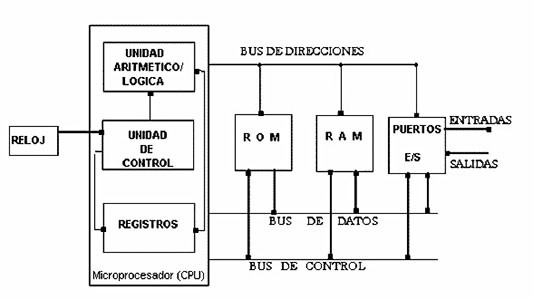
\includegraphics[height=4cm]{MicroprocesadorPartes}
   \caption{Componentes del microcontrolador y Microprocesador}
   \label{fig:ComponentesMicros}
   \end{figure}
   
   
  \subsubsection{Tipos de arquitecturas computacionales}
  \textbf{\textit{Arquitectura Harvard}}\\
  Una arquitectura Harvard tiene una memoria de instrucciones y una segunda de datos. El nombre proviene de Harvard Mark 1, una computadora electromecánica la cual precargaba un programa guardado en la memoria de programa. Esta es aun utilizada para aplicaciones en las cuales se corren programas reparados, en áreas tales como procesamiento digital de señales, pero no para la computación de propósito general. La ventaja principal es el incremento del ancho de banda dual disponible, en la cual se tiene comunicación por canales separados para las instrucciones y para los datos \cite{Furber}.\\
  Esta arquitectura (Figura \ref{fig:ArqHarvard}) ofrece la posibilidad de poder acceder a una sola instrucción en un ciclo de reloj. Mientras la memoria de programa es accedida la memoria de datos está en un bus independiente y puede ser leída y escrita . esta separación de buses permite que una instrucción sea ejecutada mientras la siguiente es extraída.
   \\ \\ 
   
   \begin{figure}[h]
   \centering
   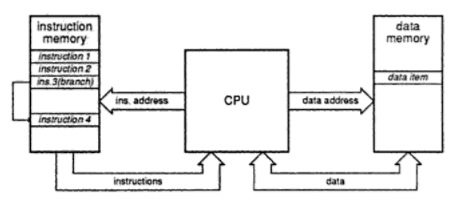
\includegraphics[height=5cm]{Harvard}
   \caption{Arquitectura Harvard \cite{Muha}.}
   \label{fig:ArqHarvard}
   \end{figure}
   
   
   \textbf{Ventajas:}
   \begin{itemize}
   	\item El tamaño de las instrucciones no está relacionado con el de los datos, y por lo tanto puede ser optimizado para que cualquier instrucción ocupe una sola posición de memoria de programa, logrando así mayor velocidad y menor longitud de programa.
   	\item El tiempo de acceso a las instrucciones puede superponerse con el de los datos, logrando una mayor velocidad en cada operación.
   \end{itemize}
   
   \textbf{\textit{Arquitectura Von Neumann}}\\
   En un sistema con arquitectura Von Neumann (Figura \ref{fig:VonNeumann}) el tamaño de la unidad de datos o instrucciones está fijado por el ancho del bus que comunica la memoria con la CPU. Así un microprocesador de 8 bits con un bus de 8 bits, tendrá que manejar datos e instrucciones de una o más unidades de 8 bits (bytes) de longitud. Si tiene que acceder a una instrucción o dato de más de un byte de longitud, tendrá que realizar más de un acceso a la memoria \cite{Camacho}. \\
   El tener un único bus hace que el microprocesador sea más lento en su respuesta, ya que no puede buscar en memoria una nueva instrucción mientras no finalicen las transferencias de datos de la instrucción anterior.
   
   \begin{figure}[htpb]
   \centering
   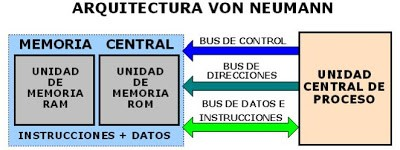
\includegraphics[height=4.8cm]{VonNeumann}
   \caption{Arquitectura Von Neumann \cite{Carva}}
   \label{fig:VonNeumann}
   \end{figure}
    
   \textbf{Limitaciones:}
   \begin{itemize}
   		\item La limitación de la longitud de las instrucciones por el bus de datos, que hace que el microprocesador tenga que realizar varios accesos a memoria para buscar instrucciones complejas.
   		\item La limitación de la velocidad de operación a causa del bus único para datos e instrucciones que no deja acceder simultáneamente a unos y otras, lo cual impide superponer ambos tiempos de acceso
\end{itemize}      
   
   \textbf{\textit{Procesador tipo RISC}}\\
   Cuando un procesador está diseñado para manejar pocas instrucciones, pero sin afectar las prestaciones del ordenador es llamada de tipo RISC que en español significa “Ordenador con Juego de Instrucciones Reducido”, esto permite programar con mucha más facilidad y, por si fuera poco, los circuitos de tipo RISC disponen de una estructura que busca como mínimo la instrucción próxima a ejecutar mientras realiza la instrucción actual. Esta estructura permite lograr no solo mayor velocidad de proceso sino también procesar cada instrucción con la misma velocidad \cite{Furber}.\\
   
   \textbf{\textit{Procesador tipo CISC}}\\
   Un procesador que permita manejar un amplio juego de instrucciones es llamado de tipo CISC que en español significa “Ordenador con Juego de Instrucciones Complejo”, programar en este tipo de arquitectura requiere en algunos casos del dominio de hasta centenares de instrucciones\cite{Jain}.
   
   \subsection{Arquitectura interna del Microcontrolador}
   Debido a que los buses se encuentran separados en la arquitectura Harvard, esta es la más utilizada en los microcontroladores actualmente.\\
   Los microcontroladores pic se basan en la arquitectura Harvard, es decir que tienen buses separados para datos e instrucciones, y su procesador es de tipo RISC, es decir, que cuenta con un número reducido de instrucciones (35 en los básicos y 70 en los más avanzados) y la mayoría de las instrucciones se ejecutan en un único ciclo de ejecución. En la memoria de programa sólo se almacena un único programa, existe una pila de hardware que almacena direcciones de regreso de funciones e incluye un potente sistema de interrupciones.
   
   \subsubsection{Componentes del microcontrolador}
   Los microcontroladores pic tienen una arquitectura RISC la cual viene con algunos estándares en la memoria on-chip (ROM), memoria RAM, memoria EEPROM, timers, ADC, USART  y puertos de entradas y salidas. Los componentes internos dependen de la familia que se elija (Figura \ref{fig:ComponentesPIC} , sin embargo, la mayoría de ellos tienen los periféricos comunes, como lo son, timers, ADC, GPIO y USART\cite{Muha}.
   
   \begin{figure}[htpb]
   \centering
   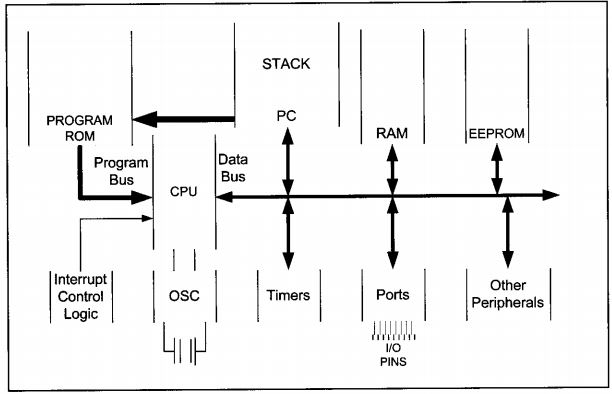
\includegraphics[height=8cm]{ComponentesPIC}
   \caption{Componentes Microcontrolador PIC \cite{Muha}.}
   \label{fig:ComponentesPIC}
   \end{figure}
   
   A continuación se explican algunos de los componentes del microcontrolador PIC:
   \begin{itemize}
   		\item \textbf{CPU:} Ejecuta las instrucciones que lee de la memoria de programa, con los datos de la memoria de datos.
   		\item \textbf{Oscilador Interno:} Genera la onda cuadrada que sincroniza el funcionamiento del microcontrolador.
   		\item \textbf{Data Memory:} Contiene los datos sobre los que trabaja el programa, así como el estado de los recursos del microcontrolador.
   		\item \textbf{Periféricos y puertos de E/S:} Recursos internos del microcontrolador como temporizadores, interrupciones, etc.
   		\item \textbf{Contador de Programa:} Guarda la posición de la siguiente instrucción a ejecutar.
   		\item \textbf{Memoria de Programa:} Guarda las instrucciones del programa a ejecutar.
   		
   \end{itemize}
   
   \subsubsection{Registros internos}
   Los microcontroladores tienen varios registros llamados registros especiales, en los cuales se alojan todas las configuraciones del microcontrolador, asi como tambien por medio de estos puertos se puede acceder a la informacion que le llega del exterior, en la Figura\ref{fig:Registros} se muestran los registros especiales internos del microcontrolador 16f887 \cite{PIC}.
   
   \begin{table}[htpb]
   \centering
   \caption{Registros Especiales 16f887 \cite{PIC}.}
   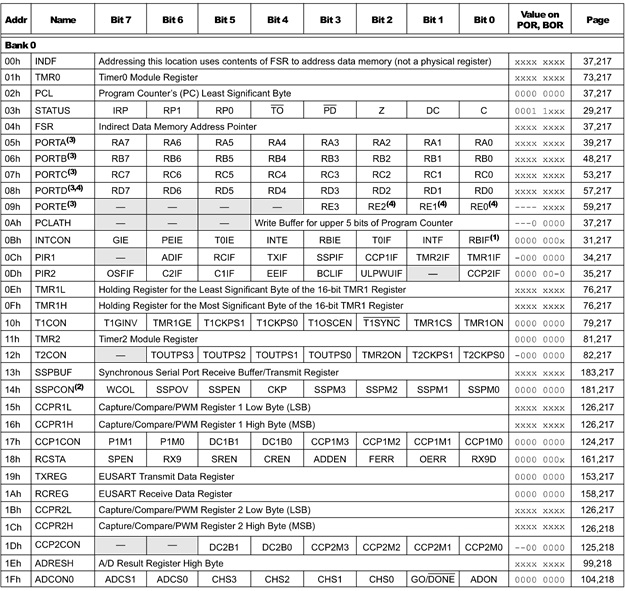
\includegraphics[height=15cm]{Registros}
   \label{fig:Registros}
   \end{table}
   
   En esta figura se puede observar la dirección de cada uno de los registros, y se observa la información que guarda cada uno de los bits del microcontrolador, es importante tener en cuenta estos registros cuando se trabaja en programación de bajo nivel.
   
   \subsubsection{Tipos y distribución de las memoria internas}
   \textbf{\textit{Memoria de Programa}}\\
   El microcontrolador está diseñado para que en su memoria de programa se almacenen todas las instrucciones del programa de control. Como éste siempre es el mismo, debe estar grabado de forma permanente. \\
   EL PIC18F4520 dispone de una memoria de programa de 32.768 bytes (0000H-7-FFFH). Las instrucciones ocupan 2 bytes (excepto las instrucciones CALL, MOVF, GOTO y LSFR que ocupan 4). Por lo tanto, la emmoria de programa puede almacenar hasta 16.384 instrucciones. \\
   Primero se almacena la parte baja de la instruccion y luego la parte alta (para las instrucciones de 4 bytes primero los bytes menos significativos y luego los mas significativos). Las instrucciones siempre empiezan en direcciones pares.\\
   
  La operacion de lectura en la posicion de memoria por encima de 7FFFH da '0' como resultado (equivalente a la instrucción NOP).\\
   Direcciones especiales de la memoria de programa:
   \begin{itemize}
   		\item Vectorizacion del Reset es 0000H
   		\item Vectorizacion de las interrupciones de alta prioridad es la 0008H
   		\item Vectorizacion de las interrupciones de baja prioridad es la 0018H
   \end{itemize}
   Estos son registros de sólo lectura y no pueden ser modificados por el usuario\cite{CCS}.
   
   \textbf{\textit{Memoria de datos}}\\
   Los datos que manejas los programas varían continuamente, y esto exige que la memoria que los contiene debe ser de lectura y escritura, por lo que la memoria RAM estática (SRAM) es la más adecuada, aunque sea volátil.\\
Hay microcontroladores que disponen como memoria de datos una de lectura y escritura no volátil, del tipo EEPROM. De esta forma, un corte en el suministro de la alimentación no ocasiona la pérdida de la información, que está disponible al reiniciarse el programa. El PIC16F84 dispone de 64 bytes de memoria EEPROM para contener datos.

   \subsection{Arquitectura externa del microcontrolador}
   El microcontrolador cuenta con diferentes periféricos que hacen posibles la interacción con el mundo exterior.
   
   \subsubsection{Distribución de terminales}
   
   En la Figura \ref{fig:TQFP} se muestra la distribución de pines de un microcontrolador 16f887 en su encapsulado TQFP, actualmente los microcontroladores son fabricados en diferentes encapsulados, dependiendo la aplicación de este es el encapsulado seleccionado.\\ 
   
   
   \begin{figure}[htpb]
   \centering
   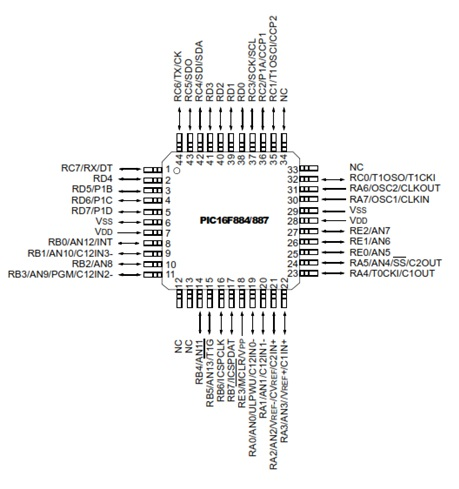
\includegraphics[height=10cm]{TQFP}
   \caption{Distribuciones de los pines en el microcontrolador 16f887 (Extraido de \cite{PIC}).}
   \label{fig:TQFP}
   \end{figure}
   
   En esta figura además de observar la distribución de las terminales, se puede observar cual es la funcionalidad de cada una de estas terminales y así en el momento de diseñar una aplicación, seleccionar correctamente cada una de los recursos del microcontrolador.
   
   \newpage
   \renewcommand{\figurename}{Figura 2.}
   \setcounter{figure}{0}
   \renewcommand{\tablename}{Tabla 2.}
   \setcounter{table}{0}
   \section{Programación de bajo nivel de microcontroladores}
   Los lenguajes de bajo nivel son aquellos en los cuales las instrucciones ejercen una acción directa con el hardware y están condicionados por la estructura física de las computadoras que lo soportan. Cuando utilizamos la palabra bajo no implica que el lenguaje sea menos potente que un lenguaje de alto nivel, sino que se refiere a la reducida abstracción entre el lenguaje y el hardware\cite{Muha}. \\
   
   La estructura de estos lenguajes es:
   \begin{itemize}
   		\item \textbf{Código Binario} - Sería la forma en la que están almacenados los programas, sea en memoria, sea en dispositivos de almacenamiento. De esta forma son recibidas y ejecutadas cada una de las instrucciones por la CPU del ordenador.
   		\item \textbf{Lenguaje Máquina} - Las invocaciones a memoria, como los procesos aritméticos lógicos son posiciones literales de conmutadores físicos del hardware en su representación booleana. Estos lenguajes son literales de tareas.
   		\item \textbf{Lenguajes ensambladores} - También denominados nemotécnicos o nemónicos, no son ya programas ejecutables directamente por el ordenador, sino textos de código fuente que necesitan de alguna herramienta para su conversión a lenguaje máquina, son los programas llamados ensambladores.
   \end{itemize}
   
   \subsection{Programación en lenguaje ensamblador}   
   Este es el único lenguaje que comprenden los microcontroladores, y es el que forma los ceros y unos del sistema binario. El lenguaje ensamblador expresa las instrucciones de una forma mas natural al hombre a la vez que muy cercana al microcontrolador, ya que cada una de estas instrucciones se corresponde con otra en código máquina.\\
   Los programas hechos en lenguaje ensamblador, al ser programado directamente sobre Hardware, son generalmente más rápidos y consumen menos recursos del sistema (memoria RAM y ROM). Al programar cuidadosamente en lenguaje ensamblador se pueden crear programas que se ejecutan más rápidamente y ocupan menos espacio que con lenguajes de alto nivel. Un programa escrito en lenguaje ensamblador consiste en una serie de Instrucciones que corresponden al flujo de órdenes ejecutables que pueden ser cargadas en la Memoria de un sistema basado en Microprocesador. \\
   El código ensamblador esta compuesto por una seria de líneas de texto, estas líneas pueden ser estructuradas en hasta cuatro campos o columnas separados por uno o mas espacios o tabulaciones entre sí.\\
   
   \textbf{Campo de etiquetas: }Expresiones alfanuméricas escogidas por el usuario para identificar una determinada línea. Todas las etiquetas tienen asignado el valor de la posición de memoria en la que se encuentra el código al que acompañan.\\
   \textbf{Campo de código: }Corresponde al nemónico de una instrucción, de una directiva o de una llamada a macro.\\
   \textbf{Campo de operandos y datos: }Contiene los operandos que precisa el nemónico utilizado. Según el código, puede haber dos, uno o ningún operando.\\
   \textbf{Campo de comentarios: }Dentro de una línea, todo lo que se encuentre a continuación de un punto y coma (;) será ignorado por el programa ensamblador y considerado como comentario.\\
   \\
   Dentro de los campos de código se puede corresponder a:
   \begin{itemize}
   		\item \textbf{Instrucciones: }son aquellos nemónicos que son convertidos por el ensamblador en código máquina que puede ejecutar el núcleo del microcontrolador. En la gama media (PIC16xxx) cada nemónico se convierte en una palabra en la memoria de programa.
   		\item \textbf{Directivas: }Pseudoinstrucciones que controlan el proceso de ensamblado del programa, pero no son parte del código. Son indicaciones al programa ensamblador de cómo tiene que generar el código máquina.
   		\item \textbf{Macros: }Secuencia de nemónicos que pueden insertarse en el código fuente del ensamblador de una manera abreviada mediante una simple llamada.
   \end{itemize}
   
   \subsubsection{Modos de direccionamiento}
   Los modos de direccionamiento indican la manera de obtener los operandos y son:
   \begin{itemize}
   \item Direccionamiento de registro
   \item Direccionamiento inmediato
   \item Direccionamiento directo
   \item Direccionamiento indirecto mediante registro
   \item Direccionamiento indirecto por registro base 
   \item Direccionamiento indexado
   \item Direccionamiento indexado respecto a una base

   \end{itemize}
   
   \textbf{\textit{Direccionamiento de registro}}\\
   Cuando ambos operando son un registro.\\
   \textit{Ejemplo:}
   \hspace{1cm} \textbf{MOV AX,BX;} transfiere el contenido de BX en AX.\\ 
   
   \textbf{\textit{Direccionamiento inmediato}}\\
   Cuando el operando origen es una constante.\\
   \textit{Ejemplo:}
   \hspace{1cm} \textbf{MOV AX,500;} carga en AX el valor 500.\\ 
    
    \textbf{\textit{Direccionamiento directo}}\\
  Cuando el operando es una dirección de memoria. Ésta puede ser especificada con su valor entre [ ], o bien mediante una variable definida previamente .\\
   \textit{Ejemplo:}
   \hspace{1cm} \textbf{MOV BX,[1000];} almacena en BX el contenido de la dirección de
memoria DS:1000.\\ 

\textbf{\textit{Direccionamiento indirecto mediante registro}}\\
  Cuando el operando está en memoria en una posición contenida en un registro (BX, BP, SI o DI). \\
   \textit{Ejemplo:}
   \hspace{1cm} \textbf{MOV AX,[BX];} almacena en AX el contenido de la dirección de memoria DS:[BX]. \\   
   
   \textbf{\textit{Direccionamiento por registro de base}}\\
  Cuando el operando esta en memoria en una posición apuntada por el registro BX o BP al que se le añade un determinado desplazamiento. \\
   \textit{Ejemplo:}
   \hspace{1cm} \textbf{MOV AX, [BP] + 2 ;} almacena en AX el contenido de la posición de memoria que resulte de sumar 2 al contenido de BP (dentro de segmento de pila). Equivalente a MOV AX, [BP + 2]. \\   
   
   \textbf{\textit{Direccionamiento indexado}}\\
  Cuando la dirección del operando es obtenida como la suma de un desplazamiento más un índice (DI, SI). \\
   \textit{Ejemplo:}
   \hspace{1cm} \textbf{MOV AX, TABLA[DI];} almacena en AX el contenido de la posición de memoria apuntada por el resultado de sumarle a TABLA el contenido de DI. \\   
   
   \textbf{\textit{Direccionamiento indexado respecto a una base}}\\
  Cuando la dirección del operando se obtiene de la suma de un registro base (BP o BX), de un índice (DI, SI) y opcionalmente un desplazamiento. \\
   \textit{Ejemplo:}
   \hspace{1cm} \textbf{MOV AX, TABLA[BX][DI];} almacena en AX el contenido de la posición de memoria apuntada por la suma de TABLA, el contenido de BX y el contenido de DI. \\   
   
   \subsubsection{Conjunto de instrucciones}
   Las instrucciones en el lenguaje ensamblador fueron diseñadas para realizar una tarea computable en un tiempo finito, así mismo, debe de ser eficaz, es decir, de alta velocidad.\\
  En la figura \ref{fig:tablaAssembler} se muestran algunas de las operaciones utilizadas en los microcontroladores PIC.
   
   \begin{table}[htpb]
    \centering
    \caption{Principales instrucciones en ensamblador. (Extraido de \cite{PIC})}
     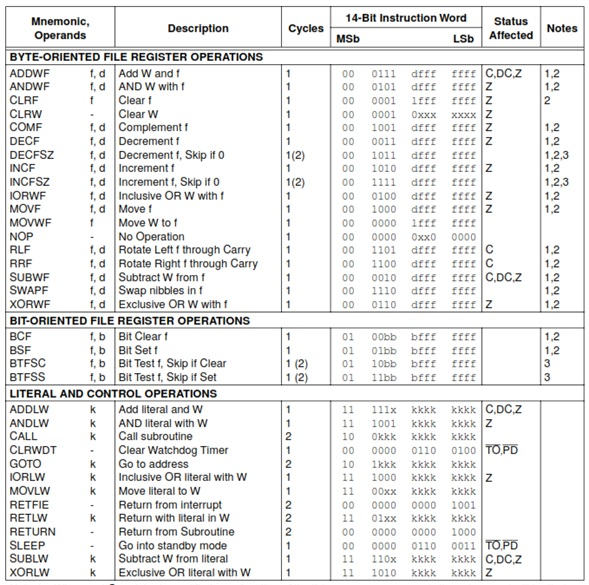
\includegraphics[height=14cm]{InstruccionesEnsamblador}
     
     \label{fig:tablaAssembler}
   \end{table}
   
   \paragraph{2.1.2.1 Instrucciones Aritméticas}
   Las instrucciones Aritméticas son una serie que nos permiten realizar algunas operaciones básicas, como lo es la suma, resta, multiplicación, división, etc.\\
     A continuación se muestran estas instrucciones y se da una breve explicación de lo que estas realizan.
     
     \begin{itemize}
     	\item ADD: suma sin acarreo
     	 \item ADC: suma con acarreo
     	 \item SUB: resta sin acarreo
     	 \item SBB: resta con acarreo
     	 \item MUL: multiplicacion sin signo
     	 \item IMUL: multiplicacion con signo
     	 \item DIV:  division sin signo
     	 \item IDIV: division con signo
     	 \item INC: incrementar
     	 \item DEC: decrementar
     	 \item NEG: cambia de signo dejando el operando en C2
     \end{itemize}
   
  \paragraph{2.1.2.2 Instrucciones lógicas}
  Los operadores lógicos realizan pruebas en expresiones lógicas. Las expresiones lógicas que se evalúan como cero o una seria vacía son falsas. \\
  Estos operadores se muestran a continuación:
  \begin{itemize}
  		\item AND
  		\item NOT
  		\item OR
  		\item XOR
  \end{itemize}
   
\paragraph{2.1.2.3 Instrucciones de control}
  Se utilizan para el control del programa, son instrucciones de salto, bucles y llamadas a procedimientos.\\
  
  \textbf{\textit{Instrucciones de salto}}\\
  Estas instrucciones permiten saltar a otras partes del código. Todas cambian el registro IP(contador de programa) y el registro CS (segmento de código) si es un salto lejano. Un salto es lejano cuando la dirección a la que se salta no está en el mismo segmento de código. Existen dos tipos de saltos: los absolutos; en lo que se especifica la dirección absoluta a la que se salta; y los relativos; que son saltos hacia delante o hacia atrás desde el valor de IP.JMP realiza un salto incondicional a la dirección especificada. La siguiente tabla relaciona los tipos de saltos y los argumentos que puede tomar esta instrucción.\\
   
   \textbf{\textit{Instrucción de llamada a procedimiento CALL y RET}}\\
   La instrucción CALL se usa para realizar una llamada a un procedimiento y la instrucción RET se usa para volver de un procedimiento. Cuando se realiza una llamada a procedimiento con CALL, se guardan en la pila el valor de IP en caso de un salto corto, y de CS e IP en caso de un salto lejano. Cuando se ejecuta la instrucción RET se recuperan de la pila los valores de IP o de CS e IP dependiendo del caso. Al salir de un procedimiento es necesario dejar la pila como estaba; para ello podemos utilizar la instrucción pop, o bien ejecutar la instrucción RET n donde n es el número de posiciones que deben descartarse de la pila.\\
   
   \textbf{\textit{Bucles}}\\
   Las instrucciones de bucle se usan para realizar estructuras repetitivas, y utilizan el registro CX como contador. LOOP esta instrucción hace que el programa salte a la dirección especificada (salto dentro del segmento), mientras que CX sea distinto de 0 y decrementa CX en 1 cada vez. \\
   Ejemplo:\\
  MOV CX,100;\\
  COMIENZO: ...\\
  ...\\
  LOOP COMIENZO; este bucle se repite 100 veces
   
\subsection{Ambiente integrado de desarrollo (IDE) para microcontroladores}   
   Un entorno de desarrollo integrado o IDE (Integrated Development Environment), es una aplicación informática que proporciona servicios integrales para facilitarle al desarrollador o programador el desarrollo de software. Normalmente, un IDE consiste de un editor de código fuente, herramientas de construcción automáticas y un depurador.\\
   Para los microcontroladores pic en lenguaje ensamblador el IDE más común es MPLAB el cual nos ofrece el servicio de compilación, programación, emulación y debuggeo de nuestro microcontrolador.
   
   \subsubsection{Ensamblador y compilador}
   MPLAB es un editor IDE gratuito, destinado a productos de la marca Microchip. Este editor es modular, permite seleccionar los distintos microcontroladores soportados, además de permitir la grabación de estos circuitos integrados directamente al programador. \\
   Dentro del IDE mplab, una vez escrito y depurado el programa, este se debe de compilar. Para esto, desde el menú Production se debe de elegir la opción build main Project (Figura \ref{fig:screnMP}) , de no existir ningún error, mplab nos devolverá un mensaje como BULD SUCCESFULL.\\
   
   \begin{figure}[htpb]
   \centering
   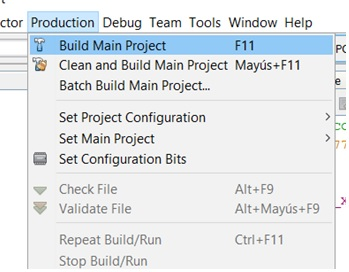
\includegraphics[height=5cm]{screenMPLAB}
   \caption{Compilar programa principal}
   \label{fig:screnMP}
   \end{figure}
   
   Dentro del compilador también es posible encontrar una serie de mensajes y advertencias; los mensajes pueden ser, por ejemplo, que se está trabajando en un banco de memoria que no es el bank 0, etc. Las advertencias tienen un poco mas de peso, por ejemplo, el PIC seleccionado no es el mismo que esta definido en el programa, etc.\\
   En ambos casos, mensajes y advertencias, la compilación termina satisfactoriamente, pero hay que tener en cuenta siempre lo que nos dices estos para prevenir errores.\\
   Una vez terminada la compilación el MPLAB generara un archivo de extensión .hex, el cual es completamente entendible para el microcontrolador PIC.
   
   \subsubsection{Simulador, debugger y emulador}
   Un simulador es un software informatico que permite la reproducción de algún sistema. Los simuladores reproducen sensaciones y experiencias que en la realidad pueden llegar a suceder. Para los microcontroladores pic existen una variedad de simuladores, de los cuales se muestran algunos a continuacion:\\
   
   \textbf{\textit{gpsim}}  \\
   gpsim es un simulador con todas las funciones para los microcontroladores pic de microchip (Figura \ref{fig:gpsim}) , el cual es distribuido bajo la licencia GNU General Public License, y algunas de sus librerías bajo la licencia GNU Lesser General Public License. Este simulador ah sido diseñado para ser lo mas preciso posible, este incluye el microcontrolador completo, desde el procesador, hasta todos los periféricos de entradas y salidas. \\
   Gpsim ha sido diseñado para ser lo mas rápido y usable posible, ya que su simulación en tiempo real de pics corriendo a 20Mhz es posible gracias a el. \\
   
   \begin{figure}[htpb]
   \centering
   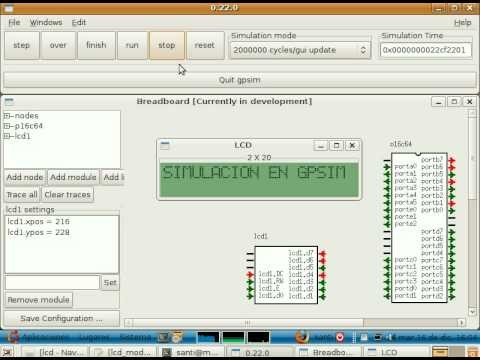
\includegraphics[height=10cm]{gpsim}
   \caption{ventana principal de GPSIM}
   \label{fig:gpsim}
   \end{figure}
   
   
   \textbf{\textit{Real Pic Simulator}}\\
   Es un simulador profesional de microcontroladores PIC (Figura \ref{fig:realPIC}) . El proceso de simulación se hace con la interacción del usuario en tiempo real a través de diferentes componentes visuales. Soporta Linux (usando Wine) y Windows. Se hace énfasis en la velocidad y el desarrollador indica que es el simulador de PICs más rápido en el mercado. Se tiene una versión de prueba de 30 días que puede ser descargada del sitio web.
   \begin{figure}[htpb]
   \centering
   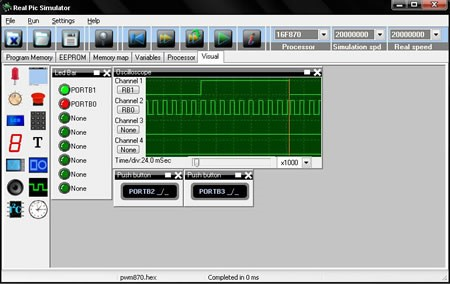
\includegraphics[height=10cm]{realPIC}
   \caption{Ventana principal de Real Pic Simulator}
   \label{fig:realPIC}
   \end{figure}
   
   \textbf{\textit{Proteus}}\\
   Uno de los simuladores mas utilizados por la comunidad estudiantil de ingeniería para circuitos digitales, es el simulador proteus, el cual nos ofrece, además de sus librerías para gran variedad de circuitos, la posibilidad de simular microcontroladores de diferentes familias como lo son AVR y PIC. \\
   En la figura \ref{fig:ssProteus} se muestra un circuito de prueba para señales de entradas y salida con el microcontrolador PIC16f887.\\
   
   \begin{figure}[htpb]
   \centering
   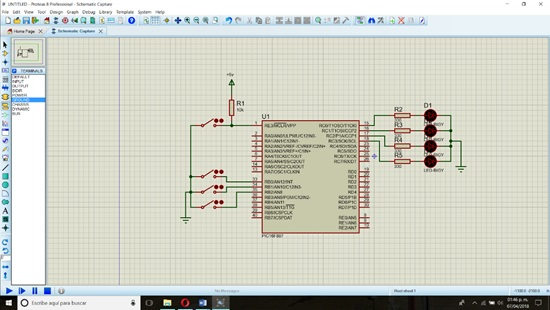
\includegraphics[height=8cm]{screenProteus}
   \caption{Simulacion de PIC16F887 en proteus}
   \label{fig:ssProteus}
   \end{figure}
   
   Un debugger o depurador es un programa el cual es utilizado para probar y eliminar errores de algún circuito o programa. MPLAB-ICD2 es un depurador para microcontroladores PIC el cual trabajo sobre el micro ya instertado dentro del circuito de la aplicación y a la vez un programador de estos dispositivos.\\
   Como debugger, el MPLAB-ICD2 permite la ejecución (controlada desde el entrono MPLAB) de programas en tiempo real y utilizando los recursos internos del propio microcontrolador pero con posibilidad de para, ejecutar paso a paso, ver el estado de los registros internos, establecer puntos de ruptura, etc.\\
   En informática, un emulador es un software que permite ejecutar programas o videojuegos en una plataforma (sea una arquitectura de hardware o un sistema operativo) diferente de aquella para el cual fueron escritos originalmente. A diferencia de un simulador, que solo trata de reproducir el comportamiento del programa, un emulador trata de modelar de forma precisa el dispositivo de manera que este funcione como si estuviese siendo usado en el aparato original.\\
   Para microcontroladores pic es mucho más común encontrarse con simuladores que con emuladores, un emulador seria emulpic.
   
   \subsubsection{Equipos programadores de Microcontroladores}
   Una vez compilado el programa y obtenido el archivo .hex, es necesario contar con un programador de microcontroladores para poder escribir el archivo hexadecimal en la memoria del microcontrolador, para esto existen diferentes programadores de diferentes compañías, los cuales se muestran a continuación.
   
   \textbf{\textit{Programador PIC K-150}}
   El K-150(Figura \ref{fig:K150}) es un programador de microcontroladores PIC por puerto USB. Dispone de un zócalo ZIF para poder realizar la programación sin dañar los pines del chip. También permite la programación en circuito ICSP con un cable provisto.
   
    \begin{figure}[htpb]
    \centering
    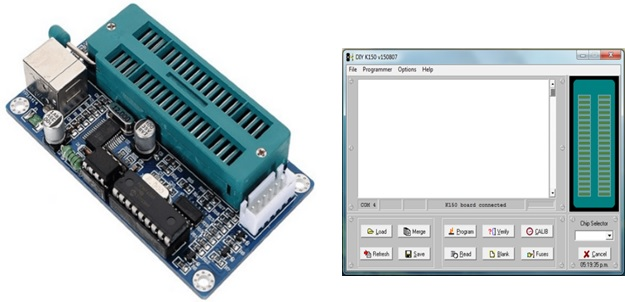
\includegraphics[height=8cm]{K150}
    \caption{Programador PIC K150}
    \label{fig:K150}
    \end{figure}
   
   Este programador soporta los microcontroladores PICs más populares de Microchip de 8 a 40 pines, la alimentación de voltaje se da por medio del puerto USB y su software de programación es muy fácil de utilizar \cite{K150}. \\
   
   \textbf{\textit{Programador PICKit 2}}\\
   Esta serie de programadores es ofrecida por microchip, El programador Pickit 2 (Figura \ref{fig:PICKIT2}) permite el uso del conector ICSP y posee conexión USB, es una herramienta de desarrollo con una interfaz fácil de usar para la programación de microcontroladores de Microchip.  Este programador es compatible con entorno de desarrollo integrado MPLAB IDE, cuenta con conexión USB y tiene la posibilidad de ser debuggeado desde el mismo software. Este programador es compatible con mas de 500 tipos de microcontroladores pic, incluyendo la familia PIC18 y PIC32 de microchip \cite{PIC}.
   
   
   \begin{figure}[htpb]
   \centering
   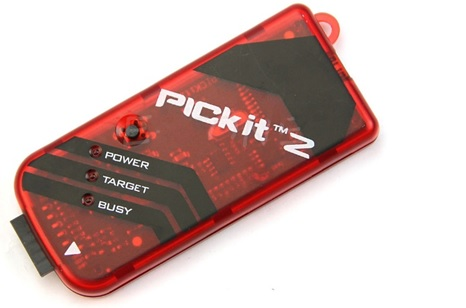
\includegraphics[height=5cm]{PICKIT2}
   \caption{Programador PICKIT 2}
   \label{fig:PICKIT2}
   \end{figure}
   
   \textbf{\textit{Programador Master PROG}}\\
   El Master Prog (Figura \ref{fig:MASTER}) es el programador de PICs USB por excelencia en universidades por su calidad y confiabilidad. El master prog es compatible con los modelos más populares de microcontroladores PIC y dsPIC como lo son el PIC16F84, PIC16F628, PIC16F877A, PIC18F2550 y el PIC18F4550. Lo cual lo hace ideal para su uso por entusiastas y profesionales que trabajan continuamente con microcontroladores PIC, sobre todo dentro de la gama más comercial.\\
   Este programador ofrece compatibilidad con Windows 7 y 8, un zócalo ZIF para la programación / lectura de microcontroladores en encapsulados DIP, asi como la posibilidad de programar los microcontroladores por medio del puerto ICSP. Ofrece auto programación y compatibilidad con algunos compiladores como MPLAB o el compilador CCS C compiler.
   
   \begin{figure}[htpb]
   \centering
   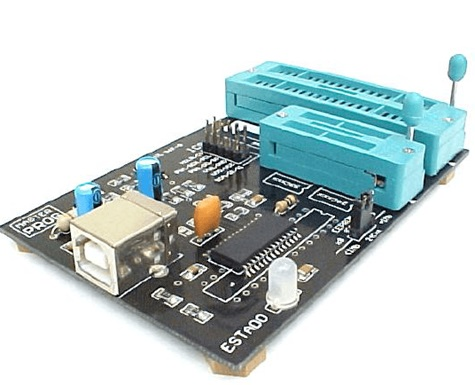
\includegraphics[height=6cm]{MASTERPROG}
   \caption{Programador Master PROG}
   \label{fig:MASTER}
   \end{figure}
   \newpage
   \renewcommand{\figurename}{Figura 3.}
   \setcounter{figure}{0}
    \renewcommand{\tablename}{Tabla 3.}
   \setcounter{table}{0}
   \section{Introducción al microcontrolador}
   Los PIC son una familia de microcontroladores desarrollados y fabricados por la empresa Microchip Technologies Inc., los cuales cuentan con una tecnología tipo RISC (Reduced Instruction Set Computer) y poseen en su arquitectura interna características especiales que varían según el modelo de PIC que deseamos utilizar.\\
   Podríamos decir que estos dispositivos se asemejan a una computadora pero de tamaño muy reducido, ya que cuentan con casi los mismos recursos que éstas, es decir, poseen memoria de programa, memoria RAM, memoria de datos, puertos de entrada o salida, temporizadores y en algunos casos cuentan con recursos adicionales como convertidores A/D, comparadores, USART (Universal Synchronous/Asynchronous Receiver/Transmitter), comunicación serie I2C, entre otros.\\
   Los microcontroladores PIC comúnmente más utilizados son los siguientes:
   \begin{itemize}
   \item PIC12C508 y PIC12C509, tienen memoria de programa EPROM, oscilador interno, y son muy utilizados en diseños de pequeños circuitos.
   \item PIC16F84A, tiene memoria de programa tipo FLASH, oscilador externo, 13 pines I/O entre otras características que estaremos estudiando a lo largo del contenido de esta obra. Este PIC ha resultado ser uno de los más populares de toda la serie.
   \item PIC16F87X, incluyen un gran número de mejoras en comparación con el PIC16F84, debido principalmente a que cuentan con un numero de pines I/O superior a éste, además de otras características relevantes. Por ejemplo, con esta serie de microcontroladores contamos con una mayor capacidad en cuanto a memoria de programa y memoria de datos.
   \item PIC18F4XX, estos microcontroladores resultan muy útiles cuando deseamos diseñar proyectos más avanzados.
   \end{itemize}
   
   \subsection{Características de la arquitectura del microcontrolador}
   Como ya se mencionó anteriormente, existen diferentes arquitecturas, sin embargo, en los microcontroladores pic y en la mayoría de los microcontroladores, la arquitectura utilizada es la arquitectura Harvard.
   
   \subsubsection{Configuración de los pines}
   Específicamente el microcontrolador PIC16f887 distribuye sus pines en sus diferentes encapsulados, en la figura 1.9 se muestra esta en un empaqueta TQFP, en la figura \ref{fig:DIP} se muestra esta distribución en el encapsulado DIP-40.
   
   \begin{figure}[htpb]
   \centering
   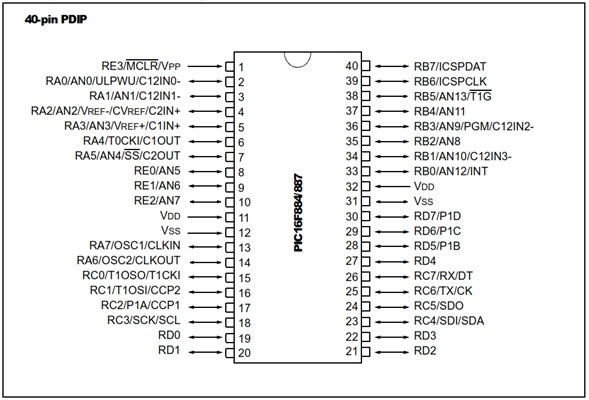
\includegraphics[height=6cm]{PIC16}
   \caption{Distribucion de pines 16F887 encapsulado DIP-40}
   \label{fig:DIP}
   \end{figure}
   
   En la figura anterior se puede observar la distribución de las terminales en el microcontrolador PIC16f887, asi mismo, se ve para que es posible utilizar cada una de estas terminales.
   
   \subsubsection{Diagrama de bloques}
   En la figura \ref{fig:DI} se muestra un diagrama de bloques de todos los componentes que contiene un microcontrolador pic.
   
   \begin{figure}[htpb]
   \centering
   \includegraphics[height=23cm]{DIAGRAMA}
   \caption{Diagrama de bloques PIC16F887 \cite{PIC}}
   \label{fig:DI}
   \end{figure}
   
   En esta figura se puede observar como es que se encuentran las memorias internas del microcontrolador, así como los periféricos de entradas y salidas, ADCs, las entradas de oscilador y su ALU.
   
   \subsubsection{Descripción de los pines}
   Cada una de las terminales del microcontrolador pic puede ser utilizado con diferentes propósitos, en el anexo 1 se muestran cada uno de los pines y las formas en las cuales pueden ser configurados estos.
   \subsection{Memorias del microcontrolador}
   Como se puede ver en la Figura \cite{DI} el microcontrolador PIC16F887 cuenta con 3 memorias, una RAM, una FLASH y una memoria tipo EEPROM.\\
   
   \textbf{\textit{Memoria RAM}}\\
   Los microcontroladores PIC tienen una serie de registros que funcionan como una RAM de propósito general. Los registros de propósito específico para los recursos de hardware disponibles dentro del propio chip también están direccionados en la RAM. La direccionalidad de la memoria varía dependiendo de la línea de dispositivos, y todos los dispositivos PIC tienen algún tipo de mecanismo de manipulación de bancos de memoria que pueden ser usados para acceder memoria externa o adicional \cite{CCS}.\\
   
   \textbf{\textit{Memoria FLASH}}
   Esta memoria, también llamada memoria de programa, es donde se almacenan todas las serias de instrucciones que realizara el microcontrolador durante su ejecución. La memoria flash derivada de las siglas EEPROM permite la lectura y escritura de múltiples posiciones de memoria en la misma operación. Gracias a ello, la tecnología flash, siempre mediante impulsos eléctricos, permite velocidades de funcionamiento muy superiores frente a la tecnología EEPROM primigenia, que sólo
permitía actuar sobre una única celda de memoria en cada operación de programación \cite{CCS}.\\

\textbf{\textit{Memoria EEPROM}}\\
Esta memoria es utilizada para guardar datos los cuales no queremos que sean borrados al reiniciar el microcontrolador, y pueden ser escritas mediante la ejecución del programa. Es un tipo de memoria ROM que puede ser programada, borrada y reprogramada eléctricamente, a diferencia de la EPROM que ha de borrarse mediante un aparato que emite rayos ultravioletas. Son memorias no volátiles.\\

\subsection{El oscilador de cristal}
Un oscilador de cristal es un oscilador electrónico que utiliza la resonancia mecánica de un cristal vibratorio de material piezoeléctrico para crear una señal eléctrica con una frecuencia precisa. Esta frecuencia es utilizada para controlar el tiempo en relojes de cuarzo, para proporcionar una señal de reloj para circuitos integrados digitales y para estabilizar las frecuencias de los transmisores y receptores de radio.\\

En los microcontroladores PIC, el oscilador de cristal externo es conectado a los pines OSC1 y OSC2 (Figura 3.3), este cristal es denominado externo por que utiliza el cristal de cuarzo aquí mencionado. Dependiendo las características de este cristal es la configuración que se debe de seleccionar en el microcontrolador, a continuación se muestra estas configuraciones para cada uno de estos tipos\cite{Muha}

   \begin{itemize}
   \item \textbf{Modo LP: }(Baja potencia) se utiliza sólo para cristal de cuarzo de baja frecuencia. Este modo está destinado para trabajar con cristales de 32.768 KHz normalmente embebidos en los relojes de cristal. Es fácil de reconocerlos por sus dimensiones pequeñas y una forma cilíndrica. Al utilizar este modo el consumo de corriente será menor que en los demás modos.
   \item \textbf{Modo XT: }se utiliza para cristales de cuarzo de frecuencias intermedias hasta 8 MHz. El consumo de corriente es media en comparación con los demás modos.
   \item \textbf{Modo HS: }(Alta velocidad) se utiliza para cristales de reloj de frecuencia más alta de 8 MHz. Al utilizar este modo el consumo de corriente será mayor que en los demas modos.
   \end{itemize}
   
   \begin{figure}[htpb]
   \centering
   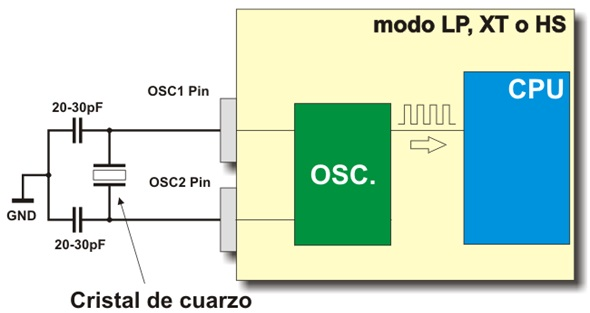
\includegraphics[height=8cm]{OSC}
   \caption{Configuracion del cristal externo del microcontrolador PIC}
   \end{figure}
   
   \subsection{Mnemónicos del microcontrolador}
   En la figura \ref{fig:tablaAssembler} se muestran algunas de las instrucciones utilizadas para programar el microcontrolador pic en lenguaje de ensamblador, a estos se les llama Mnemónicos o mnemotécnicos. 
   
   \subsection{Características físicas del chip}
   El microcontrolador PIC16F887 tiene un rango de operación de 2.0V-5.5V, un rango industrial de temperatura y un modo sleep el cual guarda energía. Existen diferentes formas en las cuales podemos encontrar un microcontrolador PIC, a continuación, se muestran algunas de estas presentaciones. Es importante destacar que el empaquetado a utilizar dependerá de la aplicación que se le dará a este.
   
   \subsubsection{PDIP-28 PIN (PLASTIC DUAL IN-LINE PACKAGE)}
   \begin{figure}[htpb]
   \centering
   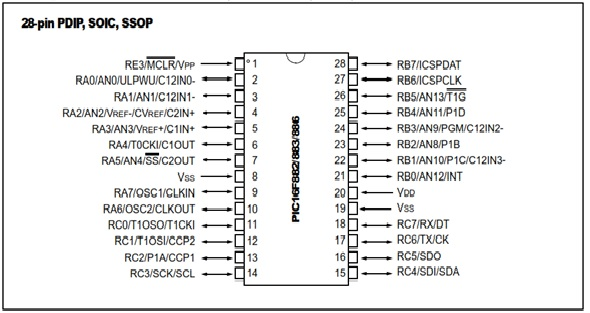
\includegraphics[height=6cm]{PDIP}
   \caption{Encapsulado PDIP}
   \label{fig:PDIP}
   \end{figure}
   
   \subsubsection{QFN-28 PIN (Quad Flat No-leads package)}
   \begin{figure}[htpb]
   \centering
   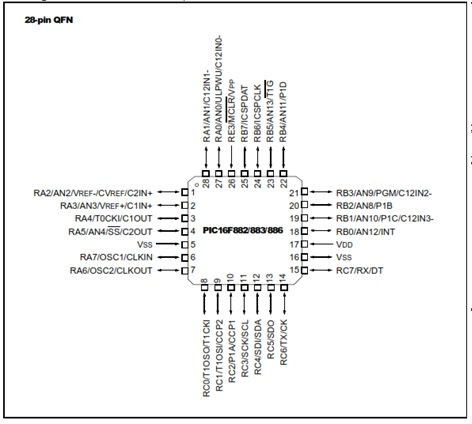
\includegraphics[height=7cm]{QFN}
   \caption{Encapsulado QFN}
   \label{fig:QFN}
   \end{figure}
   
   \subsubsection{TQFP-44 PIN (Quad Flat Package)}
   \begin{figure}[htpb]
   \centering
   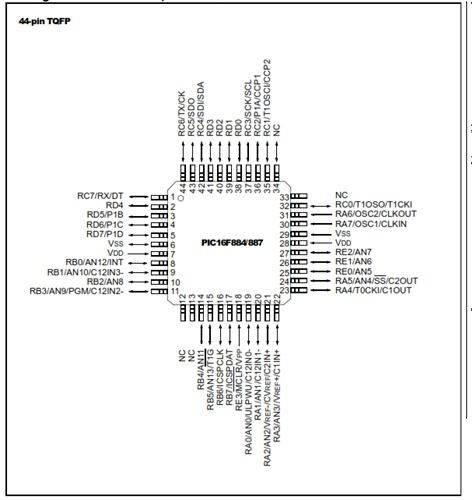
\includegraphics[height=8cm]{TQFP_2}
   \caption{Encapsulado TQFP}
   \label{fig:TQFP_2}
   \end{figure}
   \newpage
   \begin{thebibliography}{10}
     \bibitem{Ravi}\textsc{Ravi}, (2017, November 13). <<ELECTRONICS HUB,>> [Online].Available: https://www.electronicshub.org/microcontrollers-basics-structure-applications/.
     
     \bibitem{Carva}\textsc{M. Carvajal}, (2007, September 15). <<Microprocesadores y Microcontroladores,>> [Online].Available: http://microrpocesadores-blog.blogspot.mx/2007/09/diferencia-entre-microprocesadores-y.html.
     
     \bibitem{Furber}\textsc{S. B. Furber}. \textit{VLSI RISC Architecture and Organization}. New York: MARCEL DEKKER,1989.
     
     \bibitem{Camacho}\textsc{R. Camacho}, (2012, April 9). <<RCM computo Integrado,>> [Online].Available: http://rcmcomputointegrado.blogspot.mx/2012/04/arquitectura-von-neumann.html.
     
     \bibitem{Jain}\textsc{P. Jain}, (2012, December 24). <<Enginners Garage,>> [Online].Available: https://www.engineersgarage.com/articles/risc-and-cisc-architecture.
     
      \bibitem{Muha}\textsc{M. A. Mazidi, R. D. McKinlay y C. Danny}. \textit{PIC MICROCONTROLLER AND EMBEDDED SYSTEMS Using Assembly and C for PIC18}. New Jersey: Pearson,2008.
      
      \bibitem{PIC}\textsc{Microchip}. \textit{PIC16f882/883/884/886/887 Data Sheet}. Microchip Technology Inc. ,2009.
      
      \bibitem{CCS}\textsc{G. B. Eduardo}. \textit{Compilador C CCS y Simulador PROTEUS para Microcontroladores PIC}. Barcelona: Marcombo,2009.
      
       \bibitem{K150}\textsc{B. Alejandro}, (2017, September 1). <<¿Cómo usar el Programador de PIC K-150?,>> [Online].Available: https://electrocrea.com/blogs/tutoriales/como-usar-programador-de-pic-k-150.
      
    \end{thebibliography}
\end{document}